%!TEX program = xelatex
\documentclass[a4paper, 11pt]{article} % Font size (can be 10pt, 11pt or 12pt) and paper size (remove a4paper for US letter paper)

%\documentclass{article}
%\usepackage[protrusion=true,expansion=true]{microtype} % Better typography
\usepackage{graphicx} % Required for including pictures
\usepackage{wrapfig} % Allows in-line images
\usepackage{ctex}

\usepackage{mathpazo} % Use the Palatino font
\usepackage[T1]{fontenc} % Required for accented characters
\usepackage{fontspec}
\usepackage{xunicode}
\usepackage{xltxtra} 
\usepackage{amsmath}
\usepackage{geometry}
\usepackage[colorlinks,linkcolor=black]{hyperref}
\geometry{a4paper,scale=0.8}
\linespread{1.05} % Change line spacing here, Palatino benefits from a slight increase by default
%\linespread{0.5}
\makeatletter
\renewcommand\@biblabel[1]{\textbf{#1.}} % Change the square brackets for each bibliography item from '[1]' to '1.'
\renewcommand{\@listI}{\itemsep=0pt} % Reduce the space between items in the itemize and enumerate environments and the bibliography

\renewcommand{\maketitle}{ % Customize the title - do not edit title and author name here, see the TITLE block below

\begin{flushright} % Right align
{\LARGE\@title} % Increase the font size of the title

\vspace{50pt} % Some vertical space between the title and author name

{\large\@author} % Author name
\\\@date % Date

\vspace{10pt} % Some vertical space between the author block and abstract
\end{flushright}
}

%----------------------------------------------------------------------------------------
%	TITLE
%----------------------------------------------------------------------------------------

\title{\textbf{量子信息学}\\ % Title
lec 4} % Subtitle

\author{\textsc{郝琰 516021910721} % Author
\\{\textit{ACM Class,2016}}} % Institution

\date{\today} % Date
\begin{document}
\maketitle
\section{Class 1}


%A : H $\rightarrow$ H. $A^*$ is the unique linear operator such that
\subsection{$A^+$ : some review}
$A^+$:算子函数,相当于把一个算子映射为另一个算子
\subsubsection{定义、构造、唯一性}
\begin{itemize}
\item
A : H $\rightarrow$ H. $A^*$ is the unique linear operator such that
$$
(|\psi>, A|\psi >) = (A^+|\psi>, |\psi >)
$$
\item
construct
\begin{align*}
<i|A^+|i> & = (<i|A|i>)^* \\
A^+ &= \sum_{ij} (<j|A|i>)^*|i><j|
\end{align*}
\item
unique
$$
(|\psi>, A|\psi >) = (A^+|\psi>, |\psi >) = (B|\psi>, |\psi >)
$$
$$
(|\psi>, A^+|\psi >) = (|\psi>, B|\psi >)
$$
$$
(|\psi>, (A^+ - B)|\psi >) = 0
$$
$$
A^+ = B
$$
\end{itemize}

$A^+$:算子函数,相当于把一个算子映射为另一个算子

\subsubsection{一些性质(和转置性质相似)}

\begin{itemize}
	\item
	$$
	(A \bigotimes B)^+ = A^+ \bigotimes B^+
	$$
	\item
	$$
	(AB)^+ = B^+A^+
	$$
	\item
	tr()
	\item 
	det()
\end{itemize}

\subsection{补充}		

\subsubsection{tr()}
$$
tr(A) = \sum_{i = 1}^d <i|A|i>
$$
\begin{itemize}
	\item
	linear 
	$$
	tr(A+B) = tr(A)+tr(B)
	$$
	\item
	cyclic
	$$
	tr(AB) = tr(BA)
	$$
	\item f: L(H) -> C ; linear and cyclic
	$$
	f(H) = \lambda tr(H)
	$$
\end{itemize}

\subsubsection{全体线性算子构成一个希尔伯特空间}
$$
L(H) = \lbrace \mbox{A: A is linear operator over H} \rbrace
$$
$$
<A,B> = tr(A^+B)
$$

\subsubsection{Schmidt procedure}
对任意一组(n个)线性独立的向量,存在同样个数的线性正交基使得其与前者张成同样的线性空间


\subsection{idea 1: 柯西洗袜子}
$$
|<v|w>| \leq 1 \quad <v|v> = 1 \quad <w|w> = 1
$$
首先用w扩充一组标准正交基,w是这组基的第一个元素。
\begin{align*}
1 = <v|v> & = <v| \sum_{i = 1}^d |i><i| |v>\\
& = <v|w><w|v> + <v| \sum_{i = 2}^d |i><i| |v>\\
& \geq <v|w><w|v>
\end{align*}

\section{Class 2}

\subsection{idae 2:定义、变换及测量}
\begin{itemize}
\item	
H : state space; $|\psi>$ space vector.
$$
<\psi|\psi> =1 \quad |\psi> = \alpha |0> + \beta |1> 
$$
\item
$|\psi(t_)>$ and $|\psi(t_1)>$ 由一个酉变换联系
\item
measurement: $M_m$:线性算子,H->H. 
$$
P(m) = ||M_m|\psi>||^2
$$
$$
|\psi> = \frac{M_m|\psi>}{(P_m)^{\frac{1}{2}}}
$$
$$
\sum_m P(m) = 1
$$
$$
\sum_m <\psi|M_m^+M_m|\psi> = 1
$$
$$
\sum_m M_m^+M_m = 1
$$
\end{itemize}
$$
{|m>} ONS
$$
$$
M_m = ???
$$
Actually the reference 1 gives the correct answer.




%\subsubsection{idea 2(接测量)}
\subsubsection*{observable}
A is observable.
$$
A = A^+
$$
$$
A = \sum_{i = 1}^d a_i|i><i|
$$
这样A就可以通过其特征值$a_i$作为outcome进行测量
\subsubsection*{测量的平均值}
$$
<A>_{\psi} =\sum_m \lambda_m p (m) = \sum_m \lambda_m <\psi|A|\psi> = <\psi|\sum_m \lambda_mP_m|\psi> =  <\psi|A|\psi> = tr(A|\psi ><\psi|)
$$
(方差)

\subsection{idea 3:state discrimination}
$$|\psi> \in \lbrace |\psi_1>,|\psi_2>,.... \rbrace$$
比如有两种可能,为了把真实系统恢复出来,需要做测量\\
用$M_1,M_2,...$ 做测量,把结果根据一定条件进行划分。怎么可以做到精确分辨?\\
\subsubsection*{正交}
$$
M_1 = |\psi_1><\psi_1|
$$
$$
M_2 = |\psi_2><\psi_2|
$$
$$
M_3 = I -  |\psi_1><\psi_1|-|\psi_2><\psi_2|
$$
either $M_1 = 1$ or $M_2 = 1$, $M_3$ does not exist.
\subsubsection*{不正交}
$$
\sum_i||M_i|\psi_i||^2 
$$
对于i 从 1 到 k ,sum 为1, 对于 i从k+1 到n,sum为1\\
则该问题可转化为
$$
\exists E_1 , E_2 \geq 0 \quad E_1+E_2 = I \quad <\psi_1|E_1|\psi_1> = 1 \quad <\psi_2|E_2|\psi_2> = 1 
$$
以上为一个伪命题,
$$
E_2|\psi_1> = 0
$$
$$
E_2 = \lambda_2|\psi_1^{\bot}><\psi_1^{\bot}|
$$
$$
E_1 = \lambda_1|\psi_2^{\bot}><\psi_2^{\bot}|
$$
$$
\lambda_2|<\psi_2|\psi_1^{\bot}>| = 1
$$
$$
\lambda_2\leq 1, \quad |<\psi_2|\psi_1^{\bot}>| !=1
$$
结论不成立
\section{下节:超密集编码}



\clearpage
\section*{reference 1}
\begin{figure}[h]
        \centering
        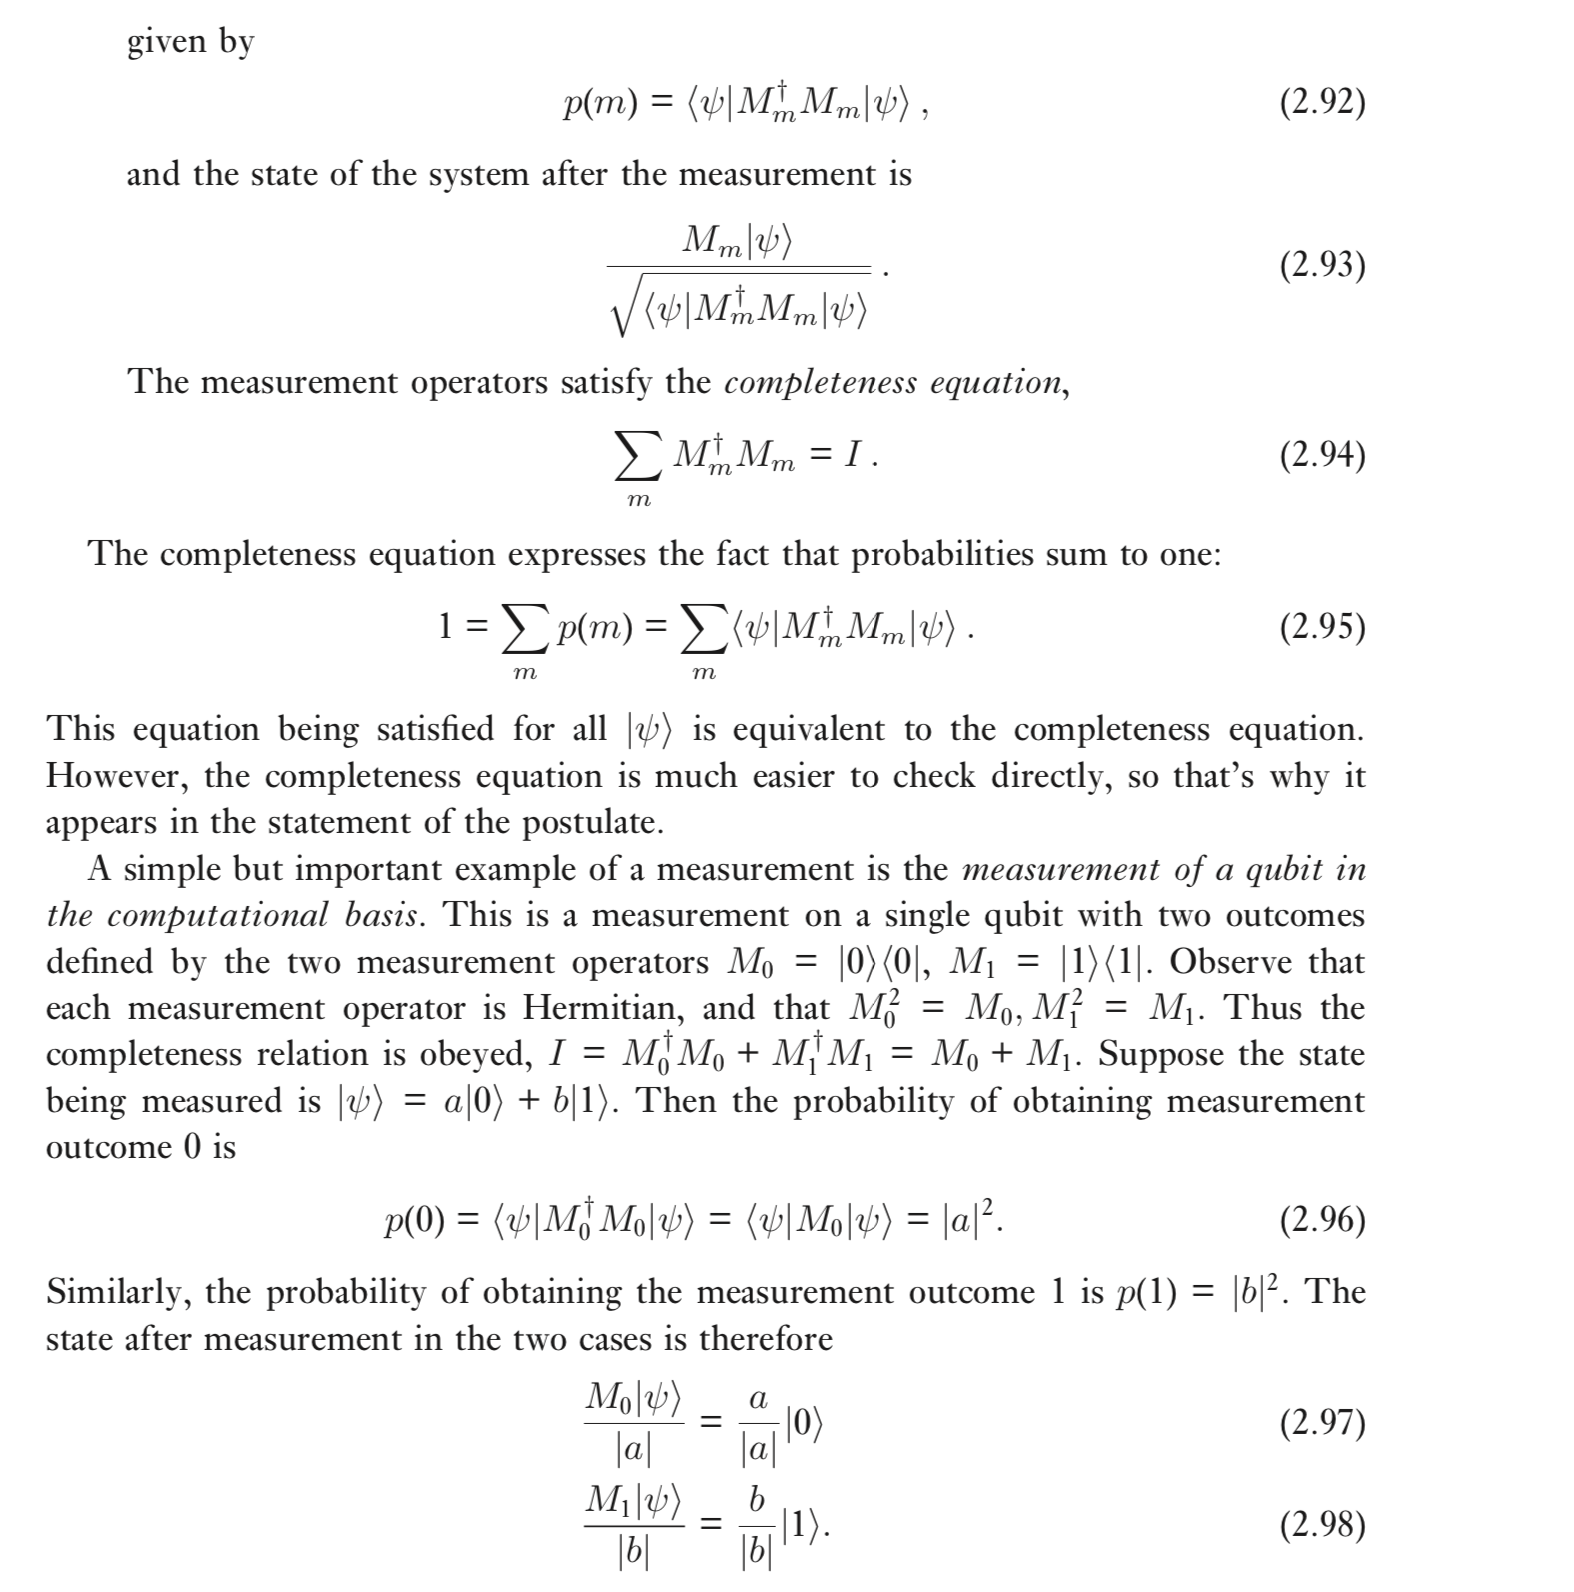
\includegraphics[width=0.99\textwidth]{2}
        \caption{approximation error graph}
\end{figure}



































\end{document}